\documentclass[12pt, a4paper]{ctexart} % 直接使用中文文档类

% ---------- 页面设置 ----------
\usepackage{algorithm}      % 算法环境
\usepackage{algorithmic}    % 算法伪代码
\usepackage{amsmath, amssymb}   % 数学公式支持
\usepackage{geometry}
\usepackage{indentfirst}   % 让首段也缩进
\usepackage{graphicx}
\usepackage{amsfonts} % 或者使用 \usepackage{amssymb}////为了使用黑体字公式
\usepackage{booktabs}%三线表格式

\setlength{\parindent}{2em} % 缩进2字符(1em≈1汉字宽度)
\geometry{left=3cm, right=2.5cm, top=2.5cm, bottom=2.5cm}

% ---------- 字体配置 ----------
\setmainfont{Times New Roman}          % 设置西文字体

% ---------- 段落格式 ----------
\linespread{1.5}                      % 1.5倍行距
\setlength{\parindent}{2em}           % 首行缩进

% ---------- 标题格式 ----------
\usepackage{titlesec}
\titleformat{\section}{\Large\bfseries\heiti}{\thesection}{1em}{}
\titleformat{\subsection}{\large\bfseries\heiti}{\thesubsection}{1em}{}

% ---------- 文档信息 ----------
\title{解读模型预测的统一方法}
\author{译者 Tinkle}
\date{\today}

\begin{document}
\maketitle{}
% ---------- 摘要页 ----------
\begin{abstract}
    在许多应用中,理解模型做出某种预测的原因与预测的准确性同样重要。然而,大型现代数据集的最高准确率往往是由复杂的模型实现的,即使是专家也很难解释这些模型,例如集合模型或深度学习模型,这就造成了准确率和可解释性之间的矛盾。为此,最近提出了各种方法来帮助用户解释复杂模型的预测结果,但往往不清楚这些方法之间的关系,也不清楚什么时候一种方法比另一种方法更可取。为了解决这个问题,我们提出了一个解释预测的统一框架,即 SHAP(SHapley Additive exPlanations)。SHAP 为每个特征分配一个特定预测的重要性值。其新颖的组成部分包括 (1) 确定了一类新的加法特征重要性度量,以及 (2) 理论结果表明,在这一类中存在一个具有一系列理想特性的唯一解决方案。这一新类别统一了六种现有方法,值得注意的是,该类别中的几种最新方法缺乏所提出的理想特性。基于从这一统一中获得的启示,我们提出了一些新方法,与以前的方法相比,这些方法的计算性能有所提高,并且/或者与人类直觉更加一致。
\end{abstract}

% ---------- 正文部分 ----------
\section{介绍}
正确解释预测模型输出结果的能力极为重要。它可以赢得用户的适当信任,为如何改进模型提供洞察力,并支持对建模过程的理解。在某些应用中,简单的模型(如线性模型)往往更容易解释,即使其准确性可能不如复杂的模型。然而,大数据的日益普及增加了使用复杂模型的益处,从而使模型输出的准确性和可解释性之间的权衡问题变得更加突出。为了解决这个问题,最近提出了多种不同的方法[5, 8, 9, 3, 4, 1]。但是,对于这些方法之间的关系以及何时一种方法优于另一种方法,我们仍然缺乏了解。 

在此,我们提出了一种新颖的统一方法来解释模型预测1 。我们的方法可能会带来三个令人吃惊的结果,从而使越来越多的方法变得更加清晰:

1. 我们引入一个视角,将对模型预测的任何解释视为模型本身,我们称之为解释模型。这样,我们就可以定义一类加法特征归因方法(第 2 节),它统一了当前的六种方法。

2. 然后,我们证明博弈论结果保证了唯一解适用于整类加法特征归因方法(第 3 节),并提出 SHAP 值作为各种方法近似的特征重要性的统一衡量标准(第 4 节)。

3. 我们提出了新的 SHAP 值估算方法,并通过用户研究证明,这些方法更符合人类的直觉,而且比现有的几种方法更能有效区分模型输出类别(第 5 节)。

\section{加法特征归因法}
简单模型的最佳解释就是模型本身;它完美地代表了模型本身,并且易于理解。对于复杂模型,如集合方法或深度网络,我们不能使用原始模型作为其本身的最佳解释,因为它不容易理解。相反,我们必须使用更简单的解释模型,我们将其定义为原始模型的任何可解释近似值。我们将在下文中说明,目前文献中的六种解释方法都使用相同的解释模型。这种之前未被重视的统一性具有有趣的意义,我们将在后面的章节中加以阐述。

设 $f$ 为待解释的原始预测模型,$g$ 为解释模型。在此,我们重点讨论 LIME [5] 中提出的基于单一输入 $x$ 解释预测 $f (x)$ 的局部方法。解释模型通常使用简化输入 $x'$,通过映射函数 $x = h_x(x')$映射到原始输入。只要 $(z') \approx (x')$,局部方法就会确保 $g(z') \approx f(h_x(z'))$。 (注意 $h_x(x′) = x$,即使$ x' $包含的信息可能比 $x$ 少,因为 $h_x$ 是针对当前输入 $x$ 的)。

定义 1 加法特征归因方法的解释模型是二元变量的线性函数:
\[
g(z') = \phi_0 + \sum_{i=1}^{M} \phi_i z'_i,
\]

$\textit{其中 } z' \in \{0,1\}^{M}, M \text{ 是简化输入特征的数量, } \phi_i \in \mathbb{R}.$

与定义 1 相匹配的解释模型方法会为每个特征归因一个效应 $\phi_i$,将所有特征归因的效应相加就近似于原始模型的输出 $f (x)$。目前许多方法都符合定义 1,下面将讨论其中几种方法。

\subsection{LIME}
LIME 方法根据围绕给定预测的局部近似模型来解释单个模型的预测[5]。LIME 使用的局部线性解释模型完全符合等式 1,因此是一种加法特征归因法。LIME 将简化输入 $x'$ 称为 “可解释输入”,映射 $x = h_x(x')$将可解释输入的二进制向量转换为原始输入空间。不同类型的 hx 映射用于不同的输入空间。对于词袋文本特征,如果简化输入为 1,则 $h_x$ 会将 1 或 0(存在或不存在)的向量转换为原始字数;如果简化输入为 0,则 $h_x$ 会将 0 转换为原始字数。对于图像,$h_x$ 将图像视为一组超级像素;然后将 1 映射为保留超级像素的原始值,将 0 映射为用邻近像素的平均值替换超级像素(这表示缺失)。

为了找到$\phi$,LIME 最小化以下目标函数:
\[
\xi = \arg\min_{g \in \mathcal{G}} L(f, g, \pi_{x'}) + \Omega(g).
\]
解释模型 $g(z')$与原始模型$ f(h_x(z'))$的忠实性是通过对简化输入空间中一组样本的损失$L$ 来实现的,损失 $L$ 由局部核 $π_x$ 加权。由于在 LIME 中,$g$ 遵循等式 1,而 $L$ 是平方损失,因此等式 2 可通过惩罚线性回归求解。

\subsection{DeepLIFT}
\textit{DeepLIFT} 最近被提出作为一种递归预测解释方法,用于深度学习 。它为每个输入 $x_i$ 赋予一个值 $C_{\Delta x_i \Delta y}$,表示该输入被设置为参考值而不是其原始值时对模型的影响。这意味着对于DeepLIFT,映射 $x = h_x(z')$ 将二进制值转换为原始输入值,其中 1 表示输入取其原始值,0 表示输入取参考值。参考值由用户选择,通常代表特征的无信息背景值。

DeepLIFT 使用一个 "求和到增量"(summation-to-delta)特性,该特性如下:
\[
\sum_{i=1}^{n} C_{\Delta x_i \Delta o} = \Delta o,
\]

其中 $o = f(x)$ 是模型输出,$\Delta o = f(x) - f(r)$,$\Delta x_i = x_i - r_i$,$r$ 是参考输入。
如果我们令 $\phi_i = C_{\Delta x_i \Delta o}$ 且 $\phi_0 = f(r)$,那么 DeepLIFT 的解释模型与公式 1 相匹配,因此它也是一种加性特征归因方法。

\subsection{逐层相关性传播(Layer-Wise Relevance Propagation, LRP)}

\textit{逐层相关性传播} 方法用于解释深度网络的预测 \cite{lrp}。Shrikumar 等人指出,该方法等价于 DeepLIFT,但所有神经元的参考激活值被固定为零。因此,$x = h_x(z')$ 仍然将二进制值转换为原始输入空间,其中 1 表示输入取其原始值,0 表示输入取参考值。逐层相关性传播的解释模型与 DeepLIFT 类似,符合公式 1。

\subsection{经典 Shapley 值估计}
已有三种方法使用合作博弈论的经典方程来计算模型预测的解释值:Shapley 回归值(Shapley regression values)、Shapley 采样值(Shapley sampling values) 和定量输入影响(Quantitative Input Influence)。

\textit{Shapley 回归值} 用于在多重共线性情况下衡量线性模型中特征的重要性。该方法需要对所有特征子集 $S \subseteq F$ 重新训练模型,其中 $F$ 是所有特征的集合。它为每个特征分配一个重要性值,该值表示该特征对模型预测的影响。为了计算这个值,分别训练两个模型:一个包含该特征 $i$($f_{S \cup \{i\}}$),另一个不包含该特征 $i$($f_S$)。然后,在当前输入 $x$ 上计算两个模型的预测差异:
$
f_{S \cup \{i\}}(x_{S \cup \{i\}}) - f_S(x_S),
$
其中 $x_S$ 代表特征子集 $S$ 的输入值。由于去除特征的效果依赖于模型中的其他特征,因此需要计算所有可能的特征子集 $S \subseteq F \setminus \{i\}$。
Shapley 值最终计算如下,它是所有可能差异的加权平均:

\[
\phi_i = \sum_{S \subseteq F \setminus \{i\}} \frac{|S|!(|F|-|S|-1)!}{|F|!} \left[ f_{S \cup \{i\}}(x_{S \cup \{i\}}) - f_S(x_S) \right].
\]

对于 Shapley 回归值,$h_x$ 将 1 或 0 映射到原始输入空间,其中 1 表示输入包含在模型中,0 表示输入被排除在模型之外。如果令 $\phi_0 = f_{\emptyset}(\emptyset)$,则 Shapley 回归值符合公式 1,因此也是一种加性特征归因方法。


\textit{Shapley 采样值} 旨在通过以下方式解释任意模型:
(1) 应用 Shapley 采样逼近公式 4,  
(2) 通过在训练数据中进行积分近似去除变量的影响。这种方法不需要重新训练模型,并允许计算比 $2^{|F|}$ 更少的差异。因此,Shapley 采样值的解释模型形式与 Shapley 回归值相同,因此也是一种加性特征归因方法。

\textit{定量输入影响} 是一个更广泛的框架,涉及的不仅仅是特征归因。然而,该方法的一部分独立提出了一种采样逼近 Shapley 值的方案,该方案在数值上接近 Shapley 采样值。因此,它也是一种加性特征归因方法。

\section{简单属性唯一确定加性特征归因}

加性特征归因方法的一个令人惊讶的特点是,该类中的单一解满足三个理想的属性(如下所述)。虽然这些属性在经典的 Shapley 值估计方法中是熟悉的,但对于其他加性特征归因方法来说,它们之前是未知的。

第一个理想属性是\textit{局部准确性(local accuracy)}。在对特定输入 $x$ 进行原始模型 $f$ 的逼近时,局部准确性要求解释模型至少能够匹配 $f$ 在简化输入 $x'$(对应于原始输入 $x$)上的输出。

\subsection*{属性 1(局部准确性)}

\[
f(x) = g(x') = \phi_0 + \sum_{i=1}^{M} \phi_i z'_i
\]

\textit{当 $x = h_x(z')$ 时,解释模型 $g(x')$ 匹配原始模型 $f(x)$。}

第二个属性是\textit{缺失性(missingness)}。如果简化输入表示特征的存在性,那么缺失性要求在原始输入中缺失的特征不产生影响。所有在第 2 节中描述的方法都满足缺失性属性。

\subsection*{属性 2(缺失性)}

\[
z'_i = 0 \implies \phi_i = 0
\]

\textit{缺失性约束:当 $z'_i = 0$ 时,该特征没有归因权重。}

第三个属性是\textit{一致性(consistency)}。一致性属性表明,如果一个模型发生变化,使得某些简化输入的贡献增加或保持不变,而其他输入保持不变,则该输入的归因权重不会减少。

\subsection*{属性 3(一致性)} 
设 $f_x(z') = f(h_x(z'))$,并且 $z' \setminus i$ 表示设定 $z'_i = 0$。对于两个模型 $f$ 和 $f'$, 如果:

\[
f'_x(z') - f'_x(z' \setminus i) \geq f_x(z') - f_x(z' \setminus i)
\]

\textit{对于所有 $z' \in \{0,1\}^M$,那么 $\phi_i(f',x) \geq \phi_i(f,x)$。}

\subsection*{定理 1}
\textit{仅有一个可能的解释模型 $g$ 满足定义 1 并符合属性 1、2 和 3:}

\[
\phi_i(f, x) = \sum_{z' \subseteq x'} \frac{|z'|!(M - |z'| -1)!}{M!} \left[ f_x(z') - f_x(z' \setminus i) \right]
\]

其中 $|z'|$ 表示 $z'$ 中非零项的数量,$z' \subseteq x'$ 代表所有 $z'$ 向量,其中非零项是 $x'$ 中非零项的子集。

定理 1 由合作博弈论的结合结果得出,其中值 $\phi_i$ 被称为 Shapley 值 \cite{shapley}. Young (1985) 证明了 Shapley 值是唯一满足局部准确性(属性 1)、缺失性(属性 2)和一个额外冗余属性的归因方法(见补充材料)。在该环境下,我们证明该冗余属性是多余的。属性 2 的引入是为了确保 Shapley 值适用于加性特征归因方法。

在给定的简化输入映射 $h_x$ 下,定理 1 说明在该类方法中只有一个可能的加性特征归因模型。这也意味着,如果一个归因方法违反了局部准确性或一致性(第 2 节已经满足缺失性),那么它不会符合 Shapley 值的计算要求。因此,以下章节将探讨统一的方法,以防止违反属性 1 和 3 的非预期方法。

\section{SHAP(SHapley 加法解释)}
我们提出 SHAP 值作为特征重要性的统一度量。这些值是原始模型的条件期望函数的 Shapley 值,因此,它们是方程 8 的解。

\begin{figure}[h]
    \centering
    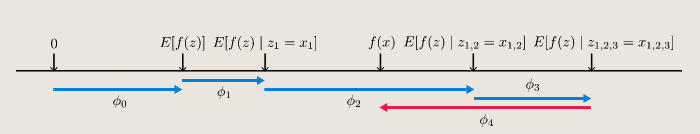
\includegraphics[width=0.9\textwidth]{img/img_1.png}
    \caption{SHAP(Shapley Additive exPlanation)值归因于每个特征在该特征条件下的期望模型预测的变化。它们解释了如何从基础值 $E[f(z)]$(即如果我们不知道任何特征时的预测值)过渡到当前的输出 $f(x)$。该图显示了单一顺序。当模型是非线性的或者输入特征不是独立的时,特征被添加到期望计算中的顺序会影响 SHAP 值,因此 SHAP 值是所有可能顺序的加权平均。}
\end{figure}

\noindent 其中 $f_x(z') = f(h_x(z')) = E[f(z) \mid z_S]$,$S$ 是 $z'$ 中非零索引的集合(见图 1)。基于第 2 和第 3 节的讨论,SHAP 值提供了唯一的加性特征重要性度量,该度量符合属性 1-3,并使用条件期望定义简化输入。在 SHAP 值的定义中,隐含地包含了一个简化输入映射 $h_x(z') = z_S$,其中 $z_S$ 代表缺失特征的填充值。由于大多数模型无法处理输入中的任意部分缺失值,我们使用 $E[f(z) \mid z_S]$ 近似 $f(z_S)$。这种 SHAP 值的定义旨在与 Shapley 回归、Shapley 采样值和定量输入影响归因方法保持一致,同时允许与 LIME、DeepLIFT 和逐层相关性传播(Layer-wise relevance propagation)建立联系。

计算 SHAP 值是一个具有挑战性的问题。然而,通过结合现有的加性特征归因方法的研究成果,我们可以对其进行近似。我们描述了两种模型无关的近似方法:
\begin{itemize}
    \item Shapley 采样值(已知方法)
    \item Kernel SHAP(新方法)
\end{itemize}
此外,我们还描述了四种针对特定模型类型的近似方法,其中两种是新方法(Max SHAP 和 Deep SHAP)。在使用这些方法时,模型的独立性和模型的线性性是两个可选假设,可以简化期望值的计算(注意 $\bar{S}$ 代表不属于 $S$ 的特征集合):
\begin{align}
    f(h_x(z')) &= E[f(z) \mid z_S]  && \text{SHAP 解释模型的简化输入映射}  \tag{9} \\
               &= E_{z_{\bar{S}} \mid z_S} [f(z)]  && \text{对 $z_{\bar{S}}$ 取期望,条件为 $z_S$}  \tag{10} \\
               &\approx E_{z_{\bar{S}}} [f(z)]  && \text{假设特征独立性}  \tag{11} \\
               &\approx f(z_S, E[z_{\bar{S}}])  && \text{假设模型线性性}  \tag{12}
\end{align}

\subsection{模型无关的近似方法}

如果我们在逼近条件期望时假设特征独立性(见方程 11),那么 SHAP 值可以直接通过 Shapley 采样值方法或定量输入影响方法进行估计。这些方法使用经典 Shapley 值方程(方程 8)的置换版本进行采样逼近。对于每个特征归因,分别执行独立的采样估计。在计算少量输入时,这种方法是合理的,但 Kernel SHAP 方法(在第 5 节介绍)减少了对原始模型的评估次数,以获得类似的逼近精度。

\subsection*{Kernel SHAP(线性 LIME + Shapley 值)}

线性 LIME 采用线性解释模型对局部近似 $f$,其中局部是在简化的二进制输入空间中测量的。乍一看,方程 2 中 LIME 的回归形式与经典 Shapley 值(方程 8)非常不同。然而,由于线性 LIME 是一种加性特征归因方法,我们知道 Shapley 值是唯一满足属性 1-3(局部准确性、缺失性和一致性)的解。一个自然的问题是:方程 2 的解是否能够恢复 Shapley 值?答案取决于损失函数 $L$、加权核 $\pi_{x'}$ 及正则项 $\Omega$ 的选择。LIME 这些参数的选择是启发式的,因此,使用这些选择,方程 2 并不能恢复 Shapley 值。这导致局部准确性和/或一致性被破坏,从而在某些情况下导致非直观的行为(见第 5 节)。

下面我们将展示如何避免启发式地选择公式 2 中的参数,以及如何找到能恢复 Shapley 值的损失函数$ L$、加权核 $\pi_{x'}$ 和正则化项 $\Omega$。
\subsection*{定理 2(Shapley 核)}

\textit{在定义 1 下,使方程 2 的解满足属性 1-3 的特定 $\pi_{x'}$、$L$ 和 $\Omega$ 形式为:}

\[
\Omega(g) = 0,
\]

\[
\pi_{x'}(z') = \frac{(M - 1)}{\binom{M}{|z'|} |z'| (M - |z'|)},
\]

\[
L(f, g, \pi_{x'}) = \sum_{z' \in Z} \left[ f(h_x^{-1}(z')) - g(z') \right]^2 \pi_{x'}(z'),
\]

其中 $|z'|$ 是 $z'$ 中非零元素的数量。

定理 2 的证明见补充材料。

需要注意的是,当 $|z'| \in \{0, M\}$ 时,$\pi_{x'}(z') = \infty$,这强制 $\phi_0 = f_{\emptyset}(\emptyset)$,并且 $f(x) = \sum_{i=0}^{M} \phi_i$。在实践中,可以在优化过程中通过解析消除这两个变量,以避免无限权重。

由于定理 2 假设 $g(z')$ 具有线性形式,并且 $L$ 是平方损失,因此方程 2 仍然可以通过线性回归求解。因此,基于博弈论的 Shapley 值可以通过加权线性回归计算 \cite{shapley_regression}。由于 LIME 使用了一种简化输入映射,该映射等价于方程 12 给出的 SHAP 逼近,因此这使得 SHAP 值的基于回归的、模型无关的估计成为可能。联合估计所有 SHAP 值的线性回归方法比直接使用经典 Shapley 方程具有更好的计算效率(见第 5 节)。

线性回归与 Shapley 值之间的直观联系在于方程 8 是均值的差值。由于均值是数据点的最小二乘估计,因此寻找一个加权核,使加权最小二乘回归能够重新计算 Shapley 值。这导致使用启发式选择的回归方法与经典 Shapley 核在某些情况下存在明显的差异(见图 2)。

\subsection{特定模型的近似方法}

虽然 Kernel SHAP 提高了模型无关 SHAP 估计的样本效率,但如果我们将注意力集中在特定类型的模型上,则可以开发更快的特定模型近似方法。

\subsection*{线性 SHAP}
对于线性模型,如果我们假设输入特征独立性(方程 11),那么 SHAP 值可以直接从模型的权重系数中进行近似。

\textbf{推论 1(线性 SHAP)} \textit{给定一个线性模型} 
\[
f(x) = \sum_{j=1}^{M} w_j x_j + b:\quad \phi_0(f, x) = b
\]
\textit{则}
\[
\phi_i(f, x) = w_j (x_j - E[x_j])
\]
\textit{该结论来源于定理 2 和方程 11,Strumbelj 和 Kononenko也曾提出类似观点。}

\subsection*{低阶 SHAP}

由于使用定理 2 进行线性回归的计算复杂度为 $O(2^M + M^3)$,因此对于较小的 $M$,如果选择一个条件期望的近似(方程 11 或 12),则可以提高计算效率。

\begin{figure}[h]
    \centering
    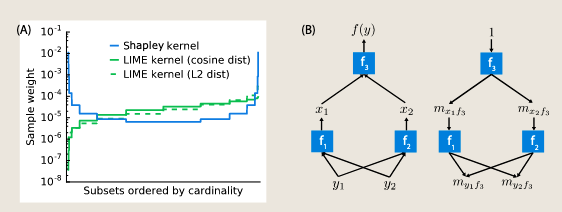
\includegraphics[width=0.9\textwidth]{./img/img_2.png}
    \caption{(A) 当所有可能的 $z'$ 向量按基数排序时,Shapley 核权重是对称的。本示例中有 $2^{15}$ 个向量。这与先前启发式选择的核不同。(B) 由多个简单组件组成的组合模型(如深度神经网络)可以使用 DeepLIFT 方式的反向传播进行快速近似计算。}
\end{figure}

\subsection*{Max SHAP}

使用 Shapley 值的置换公式,我们可以计算每个输入提高最大值的概率,而不是每个输入的所有值。按照已排序的输入值执行该计算,使得具有 $M$ 个输入的最大函数的 Shapley 值计算复杂度降低到 $O(M^2)$,而不是 $O(M^2 2^M)$。完整算法请参考补充材料。

\subsection*{Deep SHAP(DeepLIFT + Shapley 值)}

尽管 Kernel SHAP 可以用于任何模型(包括深度模型),但一个自然的问题是:是否可以利用深度神经网络的组合特性来提高计算效率?我们通过 Shapley 值和 DeepLIFT 之间的联系找到答案。

如果我们将方程 3 的参考值解释为方程 12 中的 $E[x]$,那么 DeepLIFT 在假设输入特征相互独立且深度模型为线性的情况下,近似 SHAP 值。DeepLIFT 使用线性组合规则,该规则等价于对神经网络的非线性组件进行线性化。其反向传播规则定义了如何线性化每个组件,这些规则是直观但基于启发式选择的。由于 DeepLIFT 是一种满足局部准确性和缺失性要求的加性特征归因方法,我们知道 Shapley 值是唯一满足一致性要求的归因方法。因此,这促使我们将 DeepLIFT 适配为 SHAP 值的组合近似方法,称之为 Deep SHAP。

Deep SHAP 通过将 DeepLIFT 计算得到的小型网络组件 SHAP 值递归传递,最终计算整个网络的 SHAP 值。它的计算方式如下(见图 2B):

\[
m_{x_j f_3} = \frac{\phi_i(f_3, x)}{x_j - E[x_j]}
\]
\[
\forall j \in \{1,2\}, \quad m_{y_j f_3} = \frac{\phi_i(f_j, y)}{y_i - E[y_i]}
\]
\[
m_{y_i f_3} = \sum_{j=1}^{2} m_{y_j f_j} m_{x_j f_3} \quad \text{(链式法则)}
\]
\[
\phi_i(f_3, y) \approx m_{y_i f_3} (y_i - E[y_i]) \quad \text{(线性近似)}
\]

由于简单神经网络组件的 SHAP 值可以高效地通过解析方法求解(如果它们是线性、最大池化层,或者只有一个输入的激活函数),这种组合规则使得整个模型的 SHAP 计算得到快速近似。Deep SHAP 避免了启发式选择线性化组件的需求。相反,它通过反向传播的方式从较小的 SHAP 值计算出整个模型的 SHAP 值。最大池化函数是一个示例,表明该规则在何种情况下可以提供更高效的计算方案。

\begin{figure}[h]
    \centering
    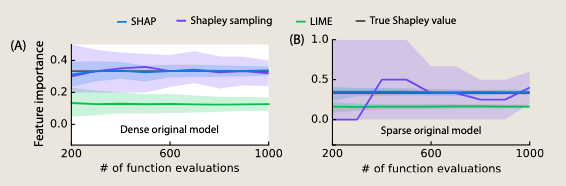
\includegraphics[width=0.9\textwidth]{./img/img_3.png}
    \caption{三种加性特征归因方法的比较:Kernel SHAP(使用去偏 Lasso)、Shapley 采样值,以及 LIME(使用开源实现)。图中显示了在两个模型中对一个特征的特征重要性估计,随着对原始模型函数的评估次数增加。200 次重复估计的第 10 和第 90 百分位数如图所示。(A) 决策树模型,使用所有 10 个输入特征来解释单个输入。(B) 决策树仅使用 100 个输入特征中的 3 个来解释单个输入。}
\end{figure}

\section{计算实验与用户研究}

我们使用 Kernel SHAP 和 Deep SHAP 近似方法评估 SHAP 值的优势。首先,我们比较了 Kernel SHAP 与 LIME 以及 Shapley 采样值的计算效率和准确性。其次,我们设计了用户研究,以比较 SHAP 值与 DeepLIFT 和 LIME 在特征重要性分配上的不同表现。正如预期的那样,SHAP 值比那些不满足第 2 节中属性 1-3 的方法更符合人类直觉。最后,我们使用 MNIST 手写数字分类任务来比较 SHAP 与 DeepLIFT 和 LIME。

\subsection{计算效率}

定理 2 通过加权线性回归将 Shapley 值与博弈论联系起来。Kernel SHAP 使用该连接计算特征重要性。这使得 SHAP 估计比以前基于采样的方程 8 估计更准确,同时减少了对原始模型的评估次数,特别是在向线性模型添加正则化时(图 3)。比较 Shapley 采样、SHAP 和 LIME 在密集(dense)和稀疏(sparse)的决策树模型中的表现,展示了 Kernel SHAP 在样本效率上的改进,同时也表明 LIME 计算的特征重要性可能与满足局部准确性和一致性的 SHAP 值存在显著差异。

\subsection{与人类直觉的一致性}

定理 1 为所有加性特征归因方法提供了一个强烈的动机,即使用 SHAP 值。LIME 和 DeepLIFT(如最初展示的那样)计算出的特征重要性值不同于 SHAP 值。为了验证定理 1 的重要性,我们使用 Amazon Mechanical Turk 进行实验,比较 LIME、DeepLIFT 和 SHAP 生成的解释与用户对简单模型的解释。我们的测试假设:优秀的模型解释应与人类对模型的理解保持一致。

我们在两个实验设置下比较了 LIME、DeepLIFT 和 SHAP 与人类解释的一致性。第一个实验使用了一种疾病评分,该评分在仅有两个症状之一存在时较高(见图 4A)。第二个实验涉及一个最大值分配问题,该问题适用于 DeepLIFT。参与者被告知一个关于三名男子如何赚钱的短故事,其中某个人的分数最高(见图 4B)。在两个实验中,参与者被要求在输入(即症状或玩家)之间分配对输出(疾病评分或赢得的金钱)的贡献。我们发现,人类解释与 SHAP 之间的匹配程度远高于其他方法。SHAP 在最大函数上的改进性能解决了 DeepLIFT 在最大池化(max pooling)函数中的已知问题。

\subsection{解释类别差异}

如第 4.2 节所讨论的,DeepLIFT 的组合方法暗示了一种 SHAP 值的组合近似(Deep SHAP)。这些见解进一步改进了 DeepLIFT,并引入了一个新的版本,以更好地匹配 Shapley 值 \cite{deeplift_shap}。

\begin{figure}[h]
    \centering
    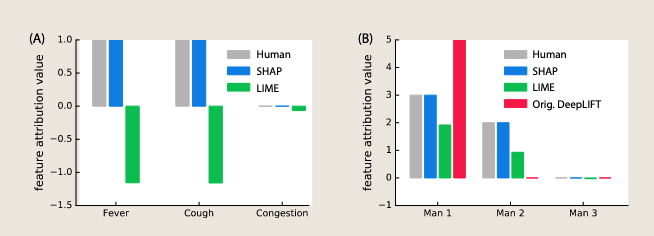
\includegraphics[width=0.9\textwidth]{./img/img_4.png}
    \caption{人类特征影响估计值显示为 30 (A) 和 52 (B) 名随机个体中最常见的解释。
    (A) 模型输出值为 2 时的特征归因(疾病评分),当发烧和咳嗽都存在时,模型输出 2;当仅有发烧或咳嗽时,输出 5;否则输出 0。
    (B) 三名男子的利润归因,基于任何一人答对最多问题的数量。第一人答对 5 道题,第二人答对 4 题,第三人未答对任何题,因此总利润为 $5$}
\end{figure}

\begin{figure}[h]
    \centering
    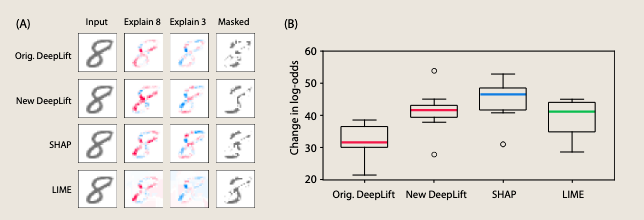
\includegraphics[width=0.9\textwidth]{./img/img_5.png}
    \caption{对 MNIST 数据集训练的卷积神经网络输出进行解释。原始 DeepLIFT 无显式 Shapley 逼近,而新的 DeepLIFT 试图更接近 Shapley 值。
    (A) 红色区域增加该类别的概率,蓝色区域降低该类别的概率。遮蔽(Masked)部分用于将 8 预测为 3。
    (B) 对 20 张随机图像进行遮蔽时,log-odds 变化表明使用更好的 SHAP 值估计的效果。}
\end{figure}

\noindent 图 5 扩展了 DeepLIFT 在卷积网络中的应用,以突出更接近 SHAP 值的估计性能提升。预训练模型和图 5 示例与中使用的相同,输入归一化到 $[0,1]$ 之间。模型包含两个卷积层、两个全连接层,并以一个 10 类 softmax 输出层结束。两种 DeepLIFT 版本都解释了线性层的归一化版本,而 SHAP(使用 Kernel SHAP 计算)和 LIME 解释整个模型的输出。

SHAP 和 LIME 都使用了 50,000 个样本进行运行(见补充材料 图 1)。为了提高表现,LIME 被修改为对单个像素区域进行分割。为与保持一致,我们选择了 20\% 的像素进行遮蔽,以根据每种方法给出的特征归因来改变预测结果,使其从 8 变为 3。

\section{结论}
模型预测的准确性和可解释性之间日益紧张的局势推动了帮助用户解释预测的方法的开发。SHAP 框架确定了加法特征重要性方法的类(包括前面的六种方法),并表明该类中存在符合所需属性的独特解决方案。SHAP 在文献中编织的统一之线是一个令人鼓舞的迹象,表明关于模型解释的共同原则可以为未来方法的开发提供信息。 我们提出了 SHAP 值的几种不同估计方法,以及表明这些值是可取的证明和实验。有希望的下一步包括开发更快的模型类型特定估计方法,做出更少的假设,整合从博弈论估计交互效应的工作,以及定义新的解释模型类。
\end{document}
